\documentclass[../../ASSD_TP1_G7.tex]{subfiles}
\usepackage{wrapfig}
\begin{document}
\chapter*{Filtro Antialiasing y Flitro Recuperador}
En el presente punto, se desglosará a continuación el proceso de análisis
y construcción de los dos filtros analógicos presentes en el trabajo
práctico y los cuales son requisito para el correcto funcionamiento
del circuito presentado. Estos filtros son el filtro Antialiasing
(conocido como FAA) y el filtro Recuperador (o filtro FR). Ambos filtros
deben presentar la configuración del tipo pasa bajos.


\section{Filtro Antialiasing}

Este filtro pasabajos es el encargado de que por medio del impedimento
del paso de ciertas frecuencias superiores a su $f_{0}$, librar de
impurezas a la señal antes de realizar una conversión analógica-digital.
Para entender de qué tipo de impurezas estamos hablando, debemos referirnos
al teorema de muestreo de Nyquist-Shannon. Este teorema demuestra
que la reconstrucción exacta de una señal periódica continua en banda
base, a partir de sus muestras, es matemáticamente posible si la señal
está limitada en banda y la tasa de muestreo es superior al doble
de su ancho de banda. Dicho de otra manera, si una señal $x_{a}(t)$
tiene como componente más alto en frecuencia $f_{max}=B$ , y la frecuencia
de muestreo cumple con que $f_{s}>2*f_{max}=2B$, entonces $x_{a}(t)$
puede recuperarse totalmente a partir de sus muestras mediante la
convolución con la función $g(x)=\frac{sin(2\pi Bx)}{2\pi Bx}=sinc(Bx)$.

De esta forma, $x_{a}(t)$ queda expresada como:
\begin{center}
\textit{\Large{}$x_{a}(t)\sim\sum_{n=-\infty}^{\infty}x_{a}(\frac{n}{f_{s}})\cdot g(t-\frac{n}{f_{s}})$}{\Large\par}
\par\end{center}

Ahora, el problema que ocasiona el no cumplir con la frecuencia de
sampleo mayor al valor indicado previamente, queda visible cuando
se realiza el análisis de Fourier correspondiente:

Supongamos que tenemos una señal en el tiempo $x(t)$ a la cual yo
quiero digitalizar. Para ello, el primer paso es discretizar la señal,
para lo cual y haciendo uso del muestreo ideal, vamos a multiplicar
la señal por un tren periódico de deltas con un periodo $T_{s}=\frac{1}{f_{s}}$
de sampleo
\begin{center}
\textit{\Large{}$\delta_{T_{s}}(t)=\sum_{n=-\infty}^{\infty}\delta(t-nT_{s})\rightarrow\tilde{x}(t)=x(t)\cdot\delta_{T_{s}}(t)$}{\Large\par}
\par\end{center}

si ahora le aplicamos la transformada de Fourier a dicha señal, obtendremos
lo siguiente:
\begin{center}
{\Large{}$\mathcal{F}\{\tilde{x}(t)\}(f)=X(f)*\delta_{T_{s}}(f)$}{\Large\par}
\par\end{center}

\begin{center}
\textit{\footnotesize{}siendo $X(f)$ y $\delta_{T_{s}}(f)$ las transformadas
de Fourier de $x(t)$ y $\delta_{T_{s}}(t)$ respectivamente. }{\footnotesize\par}
\par\end{center}

Si analizamos la función resultante en el espectro de manera gráfica,
podemos llegar a la conclusión de que el espectro que aporta la señal
$x(t)$, se va a ver repetido a lo largo de cada $\delta$ perteneciente
a $\delta_{T_{s}}(t)$. Si la frecuencia $f_{s}$ aumenta, la separación
entre $\delta$ disminuye, lo que produce una superposición de espectros.
A esa superposición de espectros se la conoce como aliasing y es lo
que se desea evitar.

Como la frecuencia de muestreo $f_{s}$ es fija, la función del filtro
pasabajos es limitar a todas aquellas frecuencias que no lleguen a
cumplir el criterio de Nyquist-Shannon y que pueda llegar a poseer
nuestra señal. Por ende, la frecuencia de corte de nuestro filtro
pasabajos queda conformada de la siguiente manera: $f_{c}=\frac{f_{s}}{2}$.


\begin{wrapfigure}{r}{0.5\columnwidth}%
\begin{centering}
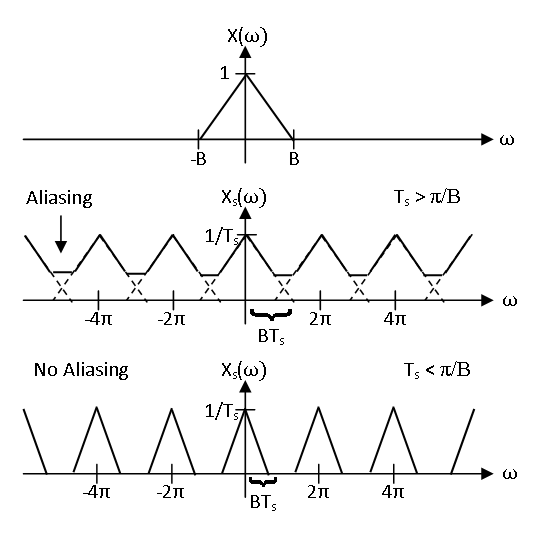
\includegraphics[scale=0.6]{Imagenes/aliasing}\caption{Efecto de aliasing de una señal.}
\par\end{centering}
\end{wrapfigure}%

\newpage


\section{Filtro Recuperador}

El otro filtro que debemos realizar es el filtro Recuperador, encargado
de seleccionar el espectro que corresponde a la señal digitalizada
que quiero recuperar. En el análisis previo que se hizo de Fourier,
llegamos a que el espectro de la función digital se repetía a lo largo
del espacio cada $f=nf_{s}$. El problema de esto, es que esa periodicidad
del espectro de mi señal no se corresponde con el de la señal original,
por lo que para poder realizar la operación exitosa, debo ``seleccionar''
el espectro que corresponde. Aquí es donde se hace evidente la función
de este filtro, pues es el encargado que los otros espectros que no
le corresponden a mi señal original se vean atenuados. 

Como tanto el filtro antialiasing como el filtro recuperador se construyen
sobre la premisa del mismo análisis de Fourier de una señal, no solo
el espectro que posee mi señal es el mismo en ambas sino que también
producen el mismo efecto en el espectro de la misma, por lo que es
posible utilizar el mismo filtro para ambas funciones en particular
(cabe destacar que se realizaron dos filtros físicos por separado
para cada etapa descrita). 

Por último, destacamos que si bien ambos filtros poseen ganancia unitaria,
para el caso del filtro recuperador es posible usar uno con ganancias
distintas a ella producto de los efectos que se producen cuando uno
muestrea la señal de manera no ideal, lo que ocasiona que la recuperación
tenga un proceso distinto y pueda llegar a manifestar distorsiones
en términos de ganancia; pero para este caso en particular se consideraron
esos efectos como despreciables.

\begin{figure}[H]

\begin{centering}
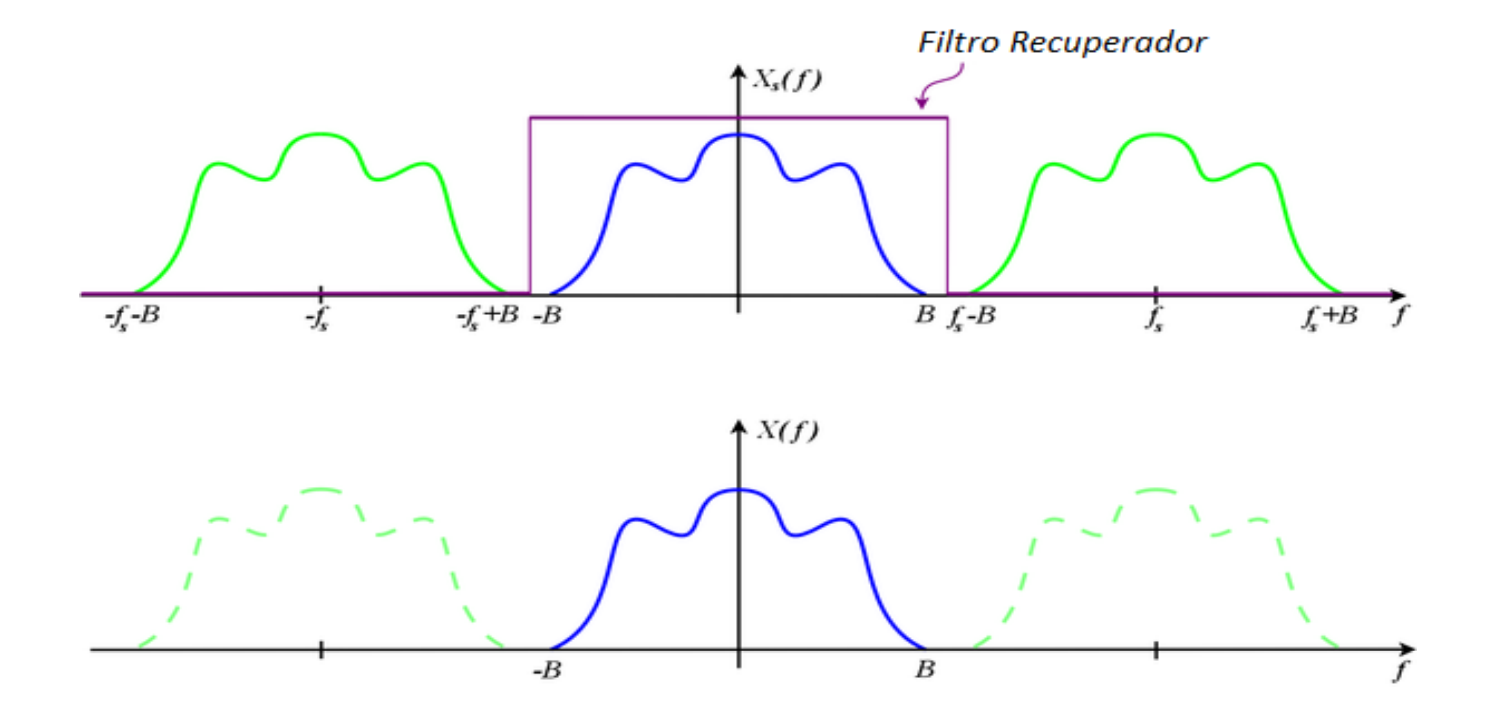
\includegraphics[scale=0.6]{Imagenes/recuperador.PNG}\caption{Filtro recuperador.}
\par\end{centering}
\end{figure}



\section{Elección de parámetros del filtro}

Teniendo en cuenta los análisis realizados previamente, queda claro
que la frecuencia del corte del filtro debe ser de la mitad de la
frecuencia de muestreo. Sin embargo, aquí surgen dos problemas principales
que son: cuál es la frecuencia de sampleo, y qué tipo de señal se
va a muestrear.

Según el tipo de señales que se deseen muestrear, cuando queremos
reconstruirla, nos encontramos con que debido a la cuantización de
la señal, hemos perdido información. 

Para entender esto de una manera más íntegra,vamos a realizar el siguiente
análisis:

Una señal cualquiera $x(t)$ a la hora de digitalizarla, termina siendo
una señal periódica de período T. Como a cualquier señal periódica,
es posible expresar su correspondiente serie de fourier en donde
\begin{center}
\textit{\Large{}$x(t)\sim\sum X_{k}\cdot e^{j2\pi f_{0}nt}$}{\Large\par}
\par\end{center}

donde $X_{k}$ son los coeficientes de la serie de Fourier que se
pueden calcular de la siguiente manera:
\begin{center}
\textit{\Large{}$X_{k}=\frac{1}{T}\int_{<T>}x(t)\cdot e^{-j2\pi f_{0}nt}dt$}{\Large\par}
\par\end{center}

entonces ahora si se le aplica la transformada de fourier a $x(t)$,
esta puede quedar expresada de la siguiente manera:
\begin{center}
\textit{\Large{}$X(f)=\sum_{k\epsilon\mathbb{Z}}X_{k}\cdot\delta(f-nf_{0})$}{\Large\par}
\par\end{center}

Esto muestra que, dependiendo las especificaciones de nuestro filtro,
va a ser posible almacenar una mayor cantidad de información de nuestra
señal para poder recuperarla. 

\begin{figure}[H]

\begin{centering}
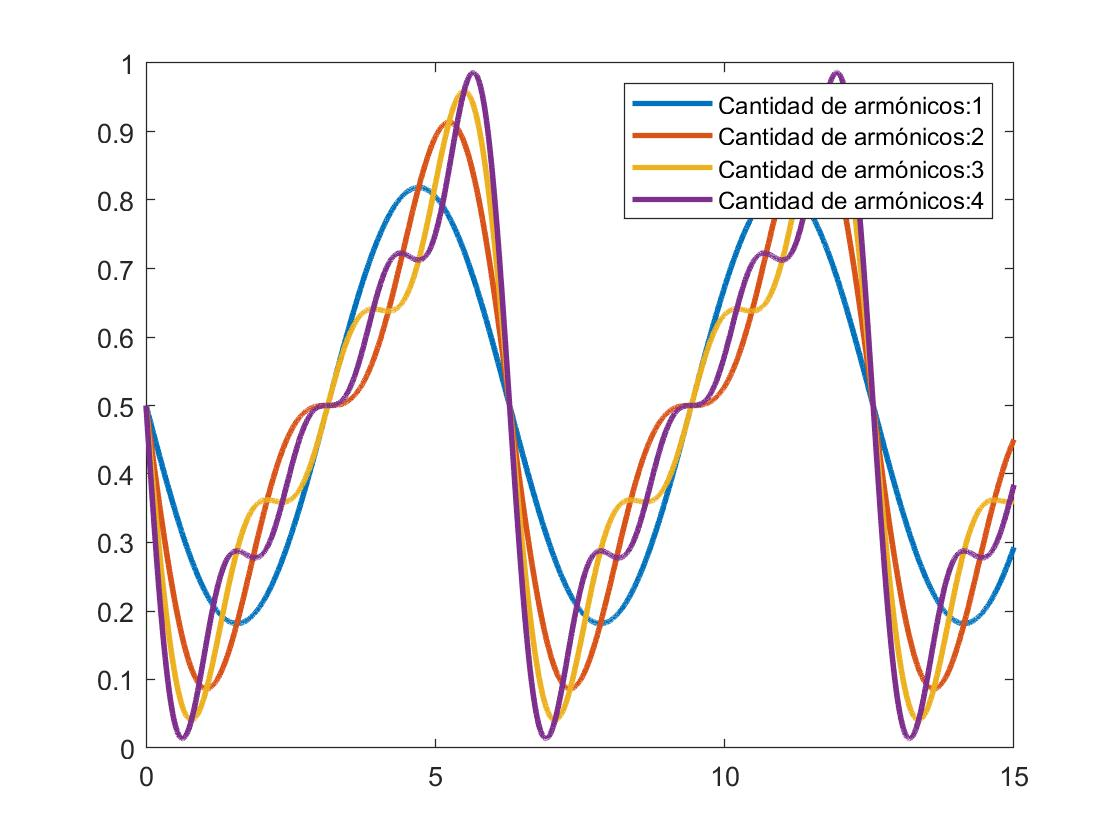
\includegraphics[scale=0.24]{Imagenes/armonicos1a4}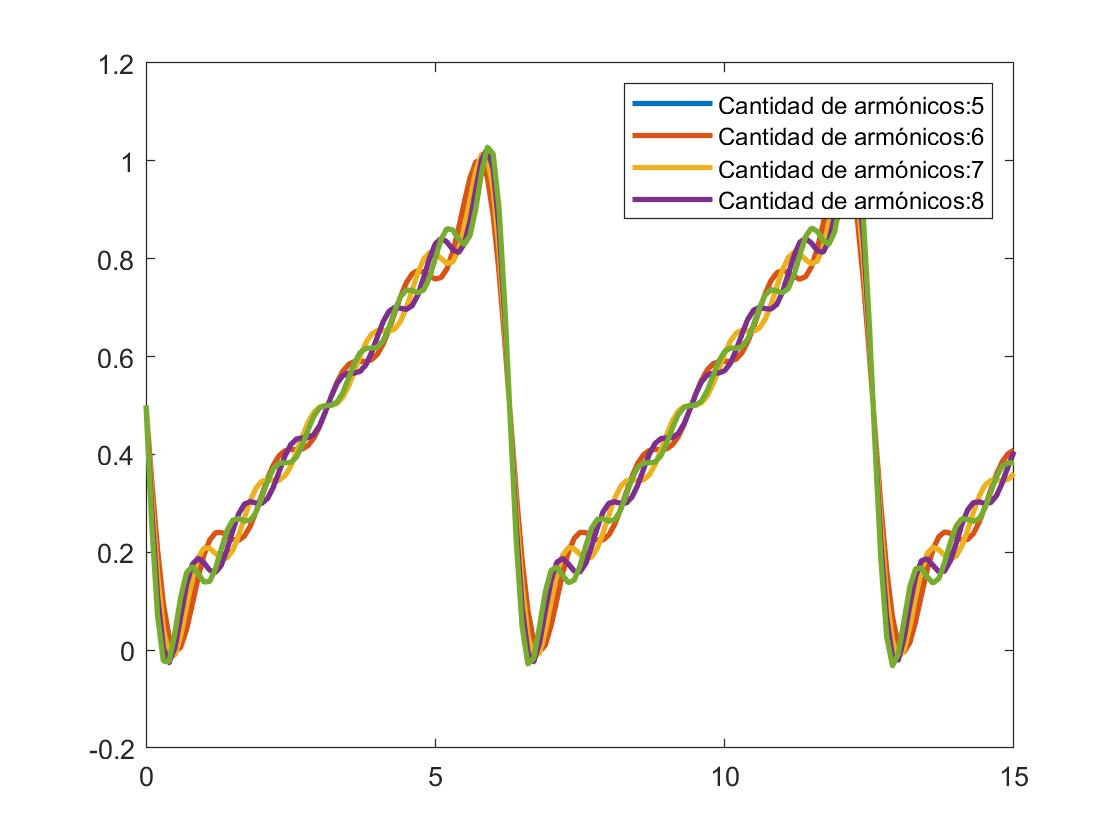
\includegraphics[scale=0.24]{Imagenes/armonicos4a8}
\par\end{centering}
\begin{centering}
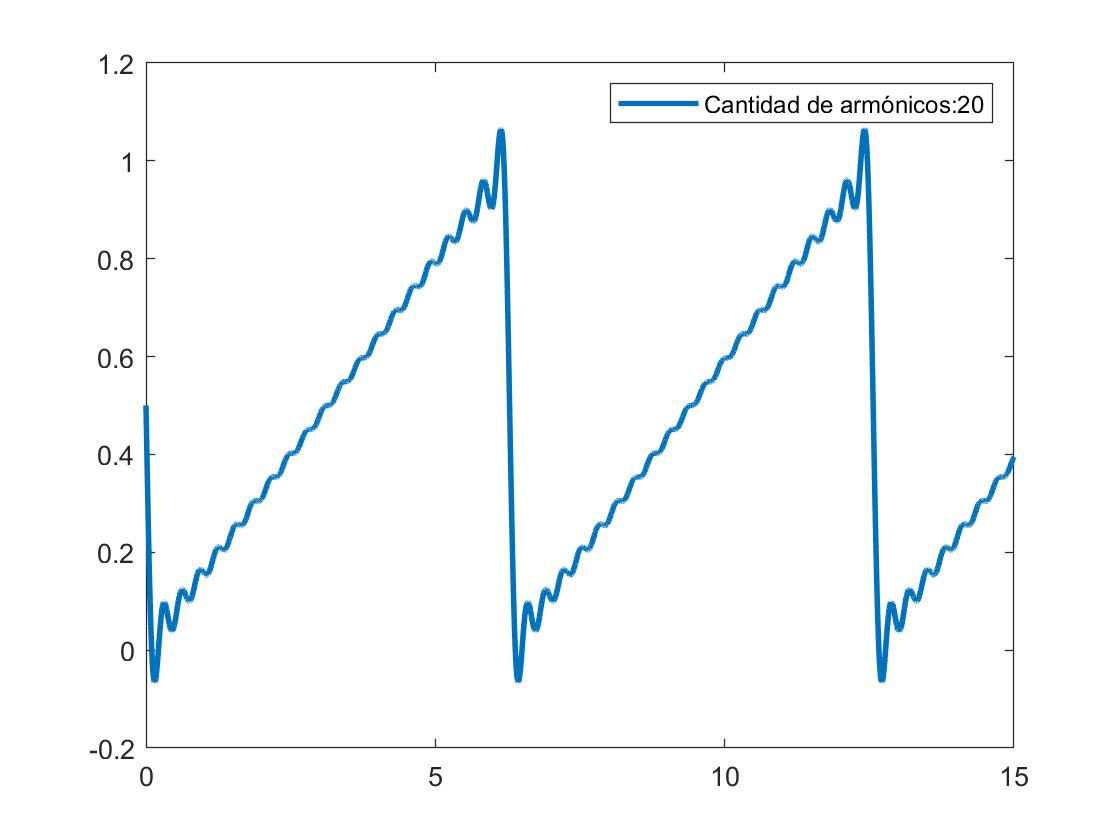
\includegraphics[scale=0.24]{Imagenes/20armonicos}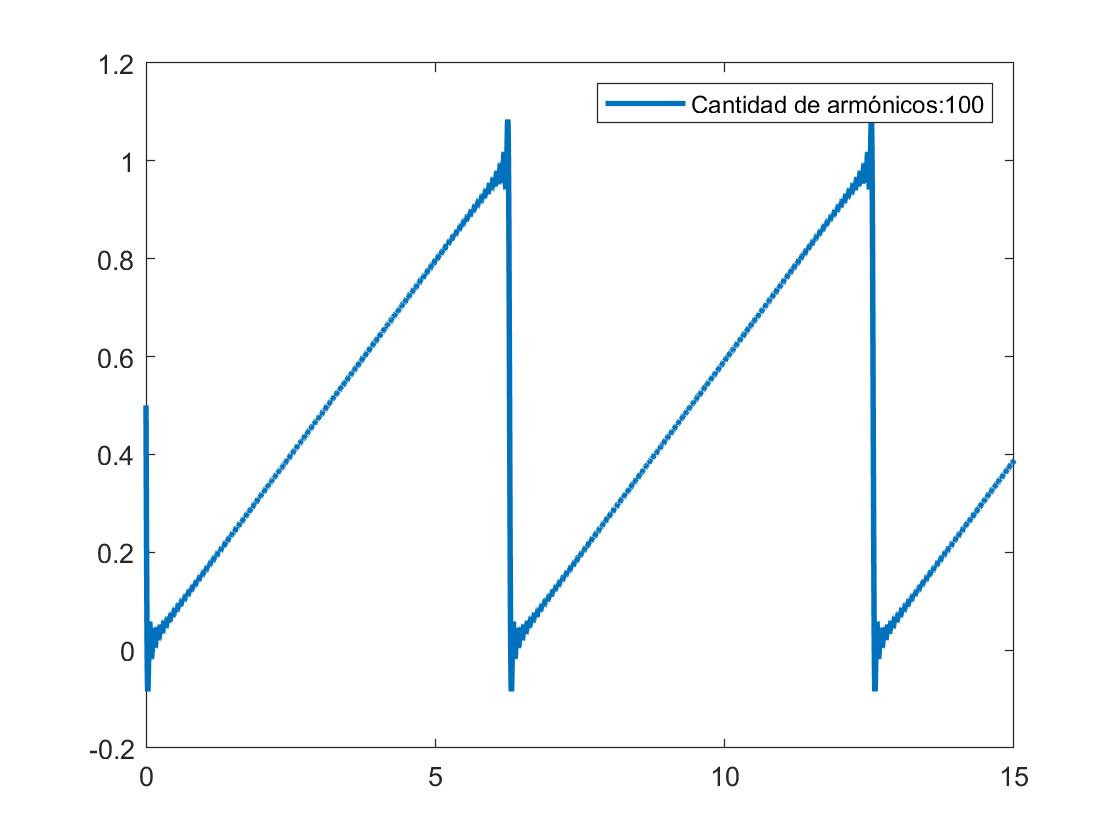
\includegraphics[scale=0.24]{Imagenes/100armonicos}\caption{Forma de una función con distinto número de armónicos.\label{fig:Forma-de-una}}
\par\end{centering}
\end{figure}

El segundo problema que se esgrime, es el hecho de la frecuencia de
sampleo que se va a utilizar. Dicha frecuencia va a ser fija, y va
a ser generada a través de un oscilador el cual si bien será explicado
en detalle más adelante, no suele alcanzar frecuencias del orden de
los kHz de frecuencia, por lo que si se desea mantener el criterio
de Nyquist-Shannon, la frecuencia de corte se va a ver limitada, y
por ende se va a ver limitada la cantidad de armónicos que se manifiesten
a traves de dichos filtros.

Al haber logrado una frecuencia del oscilador que ronda los 100kHz,
hemos podido realizar el filtro con una frecuencia de corte de 45kHz,
quedando la tabla de esta forma:

\begin{table}[H]

\begin{centering}
\begin{tabular}{|c|c|c|c|}
\hline 
$f_{p}$ & $f_{a}$ & $A_{p}$ & $A_{a}$\\
\hline 
\hline 
$45kHz$ & $67.5kHz$ & $1dB$ & $40dB$\\
\hline 
\end{tabular}\caption{Parámetros del filtro.}
\par\end{centering}
\end{table}


\section{Síntesis del Filtro}

Una vez obtenidos los parámetros característicos de nuestro filtro,
solo debemos de sintetizarlo. Para ello, vamos a elegir una aproximación
de filtros priorizando que el Q de los polos no sea excesivamente
alto, así como que tampoco lo sea el orden del mismo.

En base a estas contemplaciones, descartamos tanto las aproximaciones
de Chebycheff inverso y de Cauer para no agregar complicaciones con
los ceros de transmición que presentan dichas aproximaciones. Por
otra parte, Chebycheff se descartó por presentar ripple en la banda
pasante. También se descartaron Gauss y Bessel puesto a que como su
principal característica es el retardo lineal de fase y su banda de
transición no es la de mayor pendiente, incrementa su orden. Por lo
que nos quedan las aproximaciones de Butterworth y de Legendre. La
primera, posee la mayor planicie en la banda de paso y los Qs relativamente
pequeños; pero esto genera que el orden del filtro se incremente drásticamente.
Si se comparan los filtros obtenidos por ambas aproximaciones, el
filtro realizado con Butterworth quedaba de orden 14 con el Q más
bajo de 4.75, mientras que con Legendre el filtro quedaba en orden
8 con el Q más elevado de 6.05. Por cuestiones de simplicidad a la
hora de realizar la placa, se decidió optar por la aproximación de
Legendre. Las etapas de los filtros quedaron conformadas de la siguiente
manera:

\begin{table}[H]
\begin{centering}
\begin{tabular}{|c|c|c|}
\hline 
Etapas & Frecuencia de corte del filtro {[}Hz{]} & Q\\
\hline 
\hline 
1 & 45948.6 & 6.04\\
\hline 
2 & 39935.51 & 1.84\\
\hline 
3 & 30323.17 & 0.91\\
\hline 
4 & 21958.39 & 0.54\\
\hline 
\end{tabular}\caption{Etapas del filtro de Legendre.\label{tab:Etapas-del-filtro}}
\par\end{centering}
\end{table}


\begin{figure}[H]
\begin{centering}
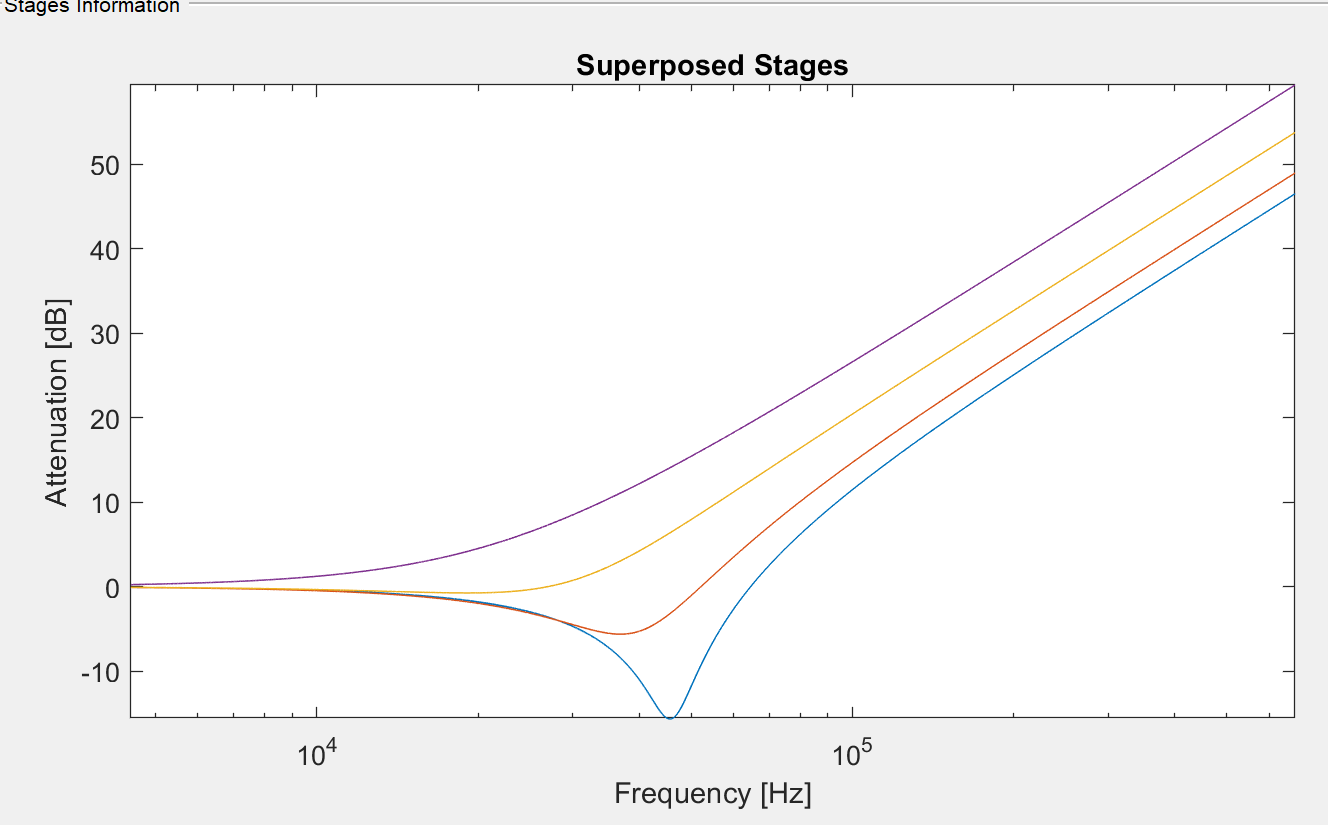
\includegraphics[scale=0.6]{Imagenes/etapas_superpuestas.PNG}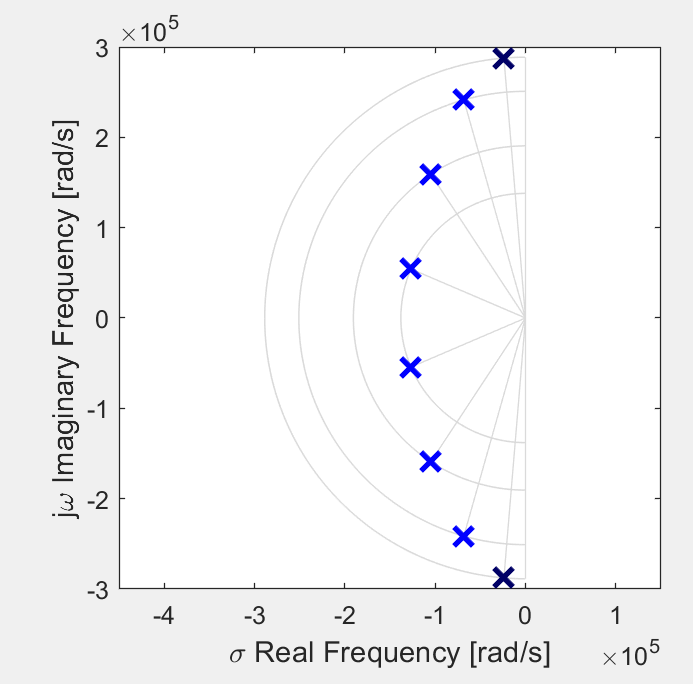
\includegraphics[scale=0.71]{Imagenes/poles_constelation.PNG}\caption{Etapas superpuestas.}
\par\end{centering}
\end{figure}


\subsection{Diseño de etapas}

Como podemos observar en la tabla \ref{tab:Etapas-del-filtro}, una
sola de las etapas posee un Q mayor a 4 mientras que el resto posee
Qs menores a 2. Es por esto que se decidió por implementar una celda
Rauch para la etapa de Q más alto, y complementar el resto de las
etapas con una topología de tipo Sallen-Key, puesto que ambas topologías
son sencillas de realizar, tienen un solo operacional, y no necesitan
calibración extrema.

\subsubsection{Celda Rauch}

Para implementar la topología Rauch de tipo pasabajos, se implementó
la siguiente planilla:
\begin{figure}[H]
\begin{centering}
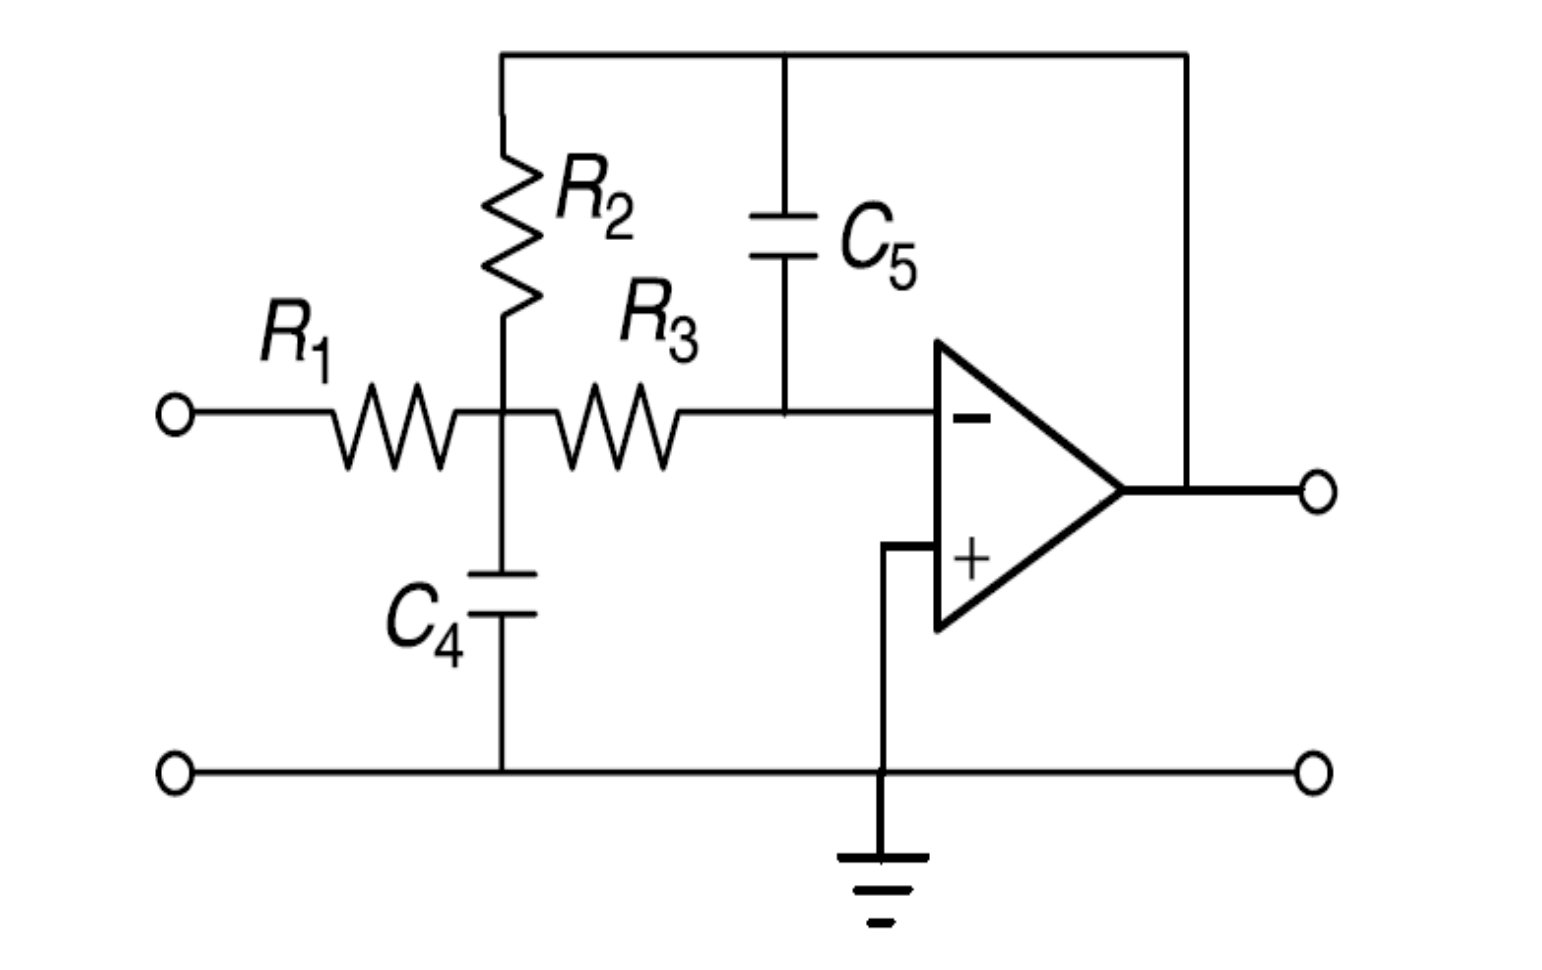
\includegraphics[scale=0.6]{Imagenes/rauch.PNG}\caption{Plantilla de la celda pasabajos Rauch.}
\par\end{centering}
\end{figure}


Para esta plantilla, las ecuaciones de diseño utilizadas fueron las
siguientes:

$\begin{cases}
\omega_{p}=\sqrt{\frac{1}{R_{2}R_{3}C_{4}C_{5}}} & \omega_{p}:frecuencia\,de\,los\,polos\\
Q_{p}=\frac{\sqrt{\frac{C_{4}}{C_{5}}}}{\frac{\sqrt{R_{2}R_{3}}}{R_{1}}+\sqrt{\frac{R_{3}}{R_{2}}}+\frac{R_{2}}{R_{3}}} & Q_{p}:factor\,de\,calidad\,de\,los\,polos\\
|H_{LP}|=\frac{R_{3}}{R_{1}} & |H_{LP}|:ganancia\,de\,la\,etapa
\end{cases}$

\subsubsection{Celda Sallen-Key}

Para implementar la topología Sallen-Key de tipo pasabajos, se implementó
la siguiente planilla:

\begin{figure}[H]
\begin{center}
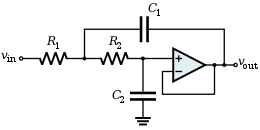
\includegraphics{Imagenes/sallen-key.png}
\end{center}
\caption{Plantilla de la celda pasabajos Sallen-Key.}
\end{figure}

Las ecuaciones del filtro pertinente a la misma son:

$\begin{cases}
\omega_{p}=\sqrt{\frac{1}{R_{1}R_{2}C_{1}C_{2}}} & \omega_{p}:frecuencia\,de\,los\,polos\\
Q_{p}=\frac{\sqrt{R_{1}R_{2}C_{1}C_{2}}}{C_{2}(R_{1}+R_{2})} & Q_{p}:factor\,de\,calidad\,de\,los\,polos
\end{cases}$

Basándonos en las ecuaciones descriptas anteriormente para cada topología,
materializamos las etapas de los filtros, igualando comonentes en
donde es posible para simplificar el diseño y armado. La simulación
del filtro final, quedó conformada de la siguiente manera:

\begin{figure}[H]
\begin{center}
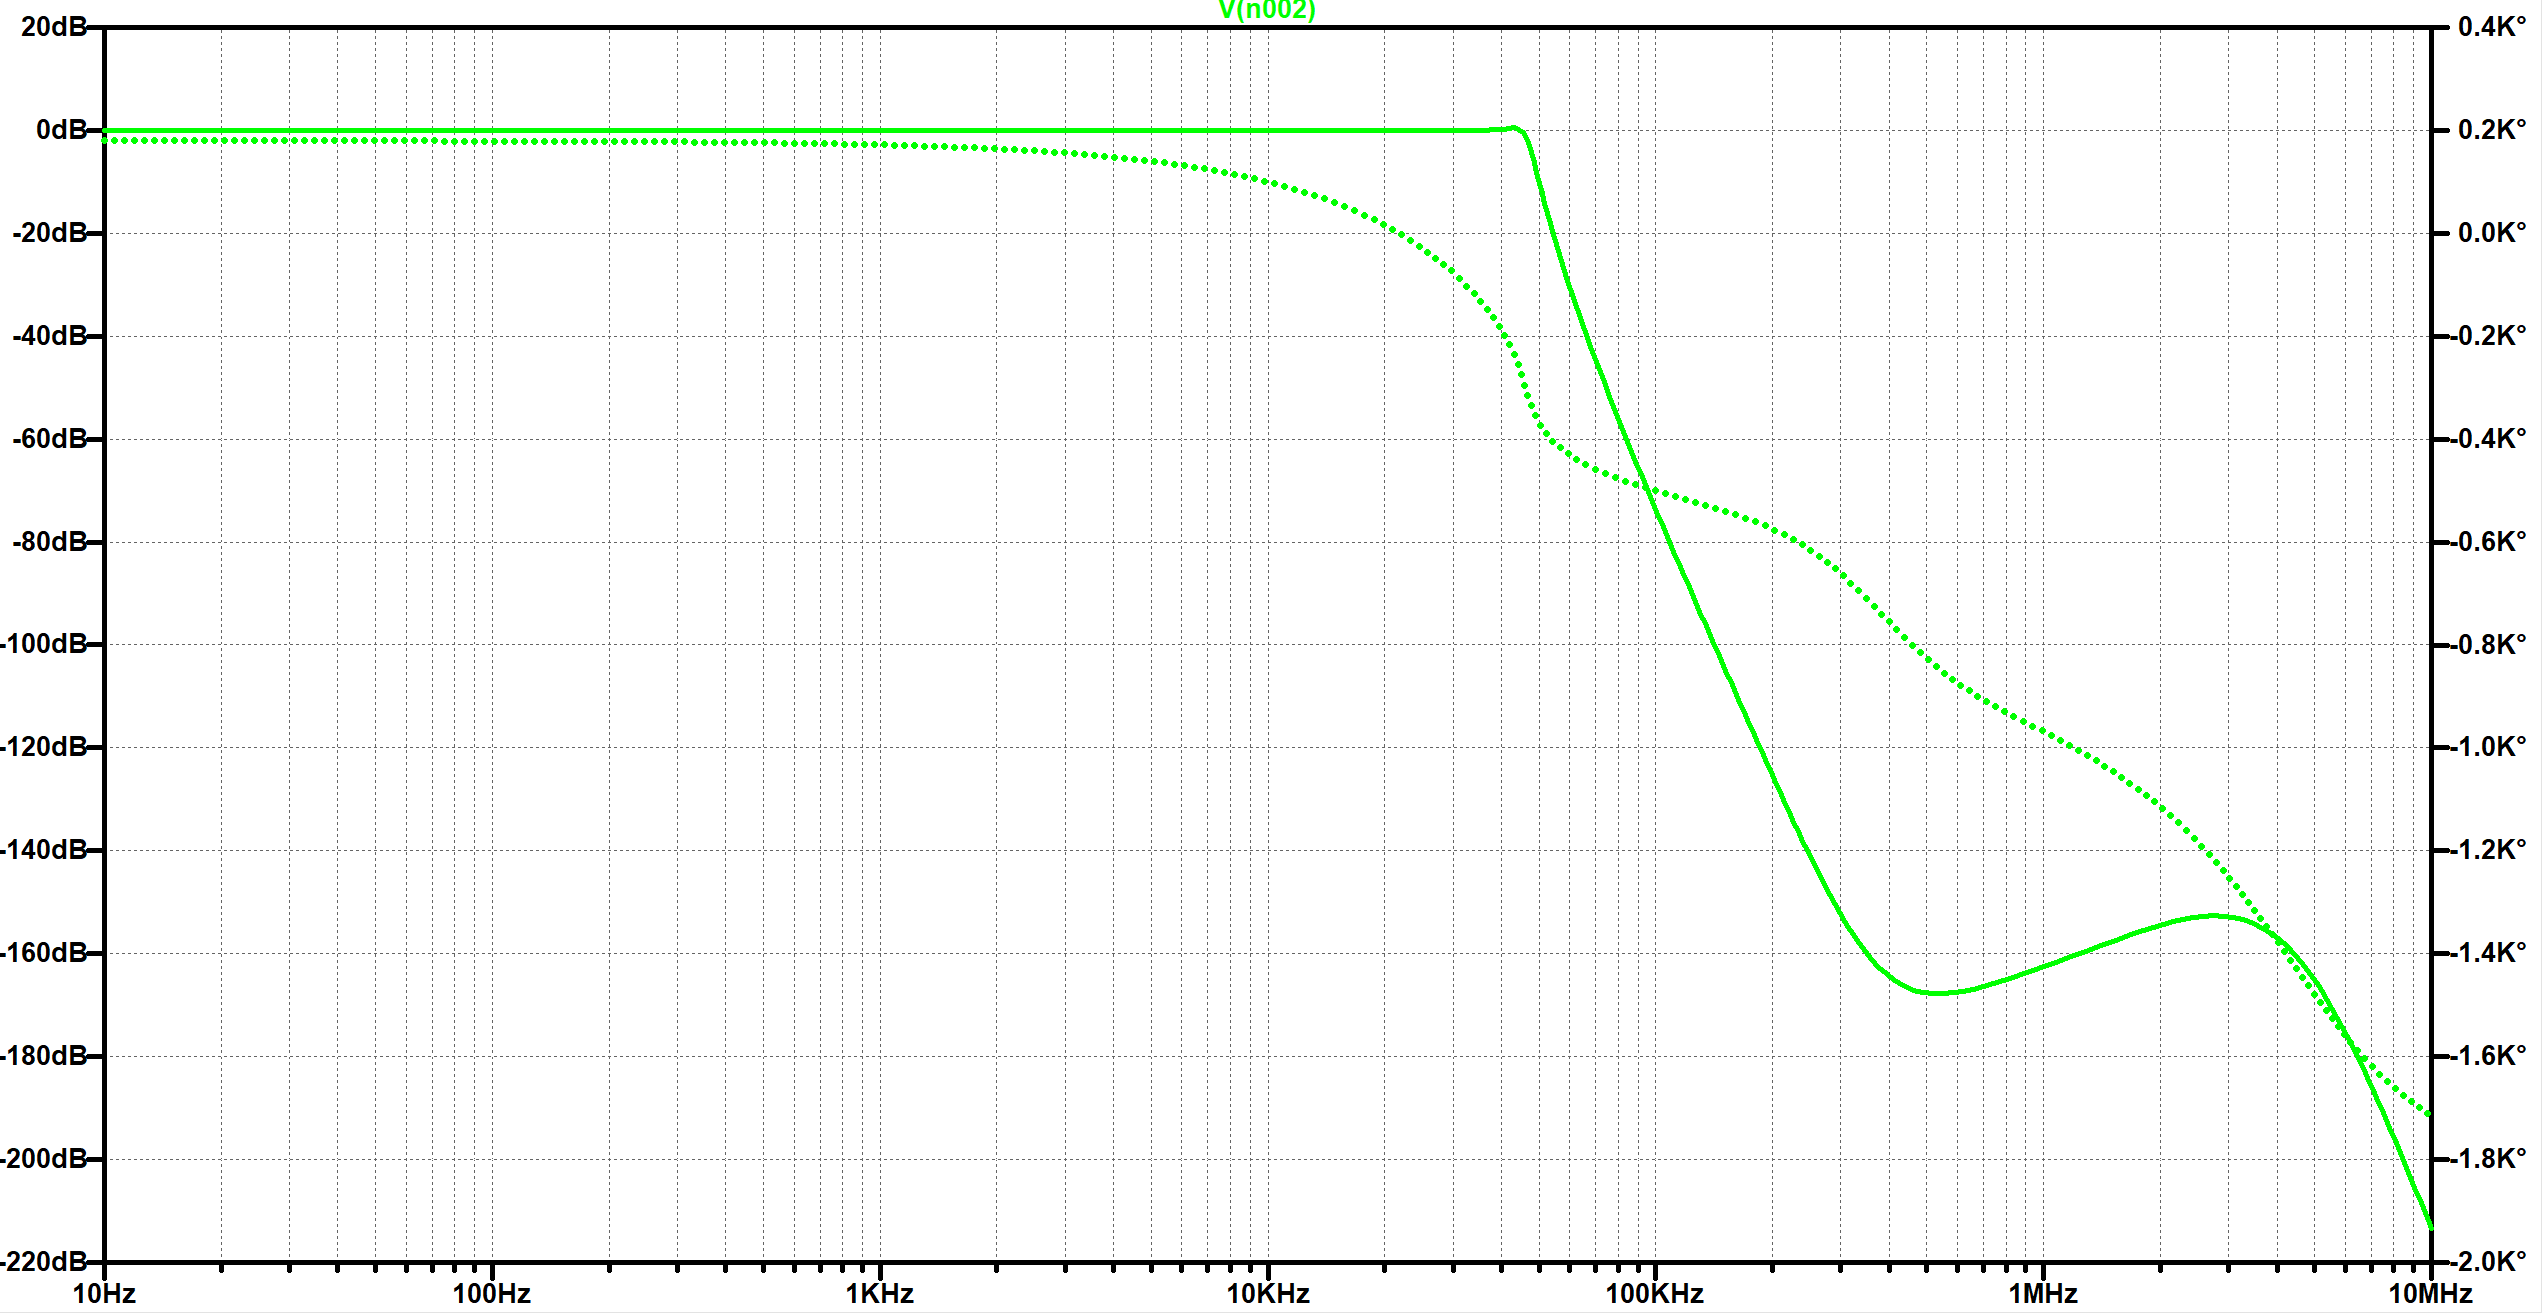
\includegraphics[scale=0.55]{Imagenes/filtroLTSpice.PNG}
\end{center}
\caption{Simulación del filtro con LTSpice.}

\end{figure}

Para realizar un análisis más profundo, se optó por realizar una simulación
montecarlo con el fin de determinar si era oportuno construir los
filtros calculados con componentes al 10\% o por el contrario eran
necesarios utilizar componentes de mayores prestaciones. A continuación
se muestran simulaciones hechas con las resistencias y capacitores
por separado tanto al 10\% como al 5\% y al 1\%. Podemos observar
los resultados en los siguientes gráficos:

\begin{figure}[H]
\begin{center}

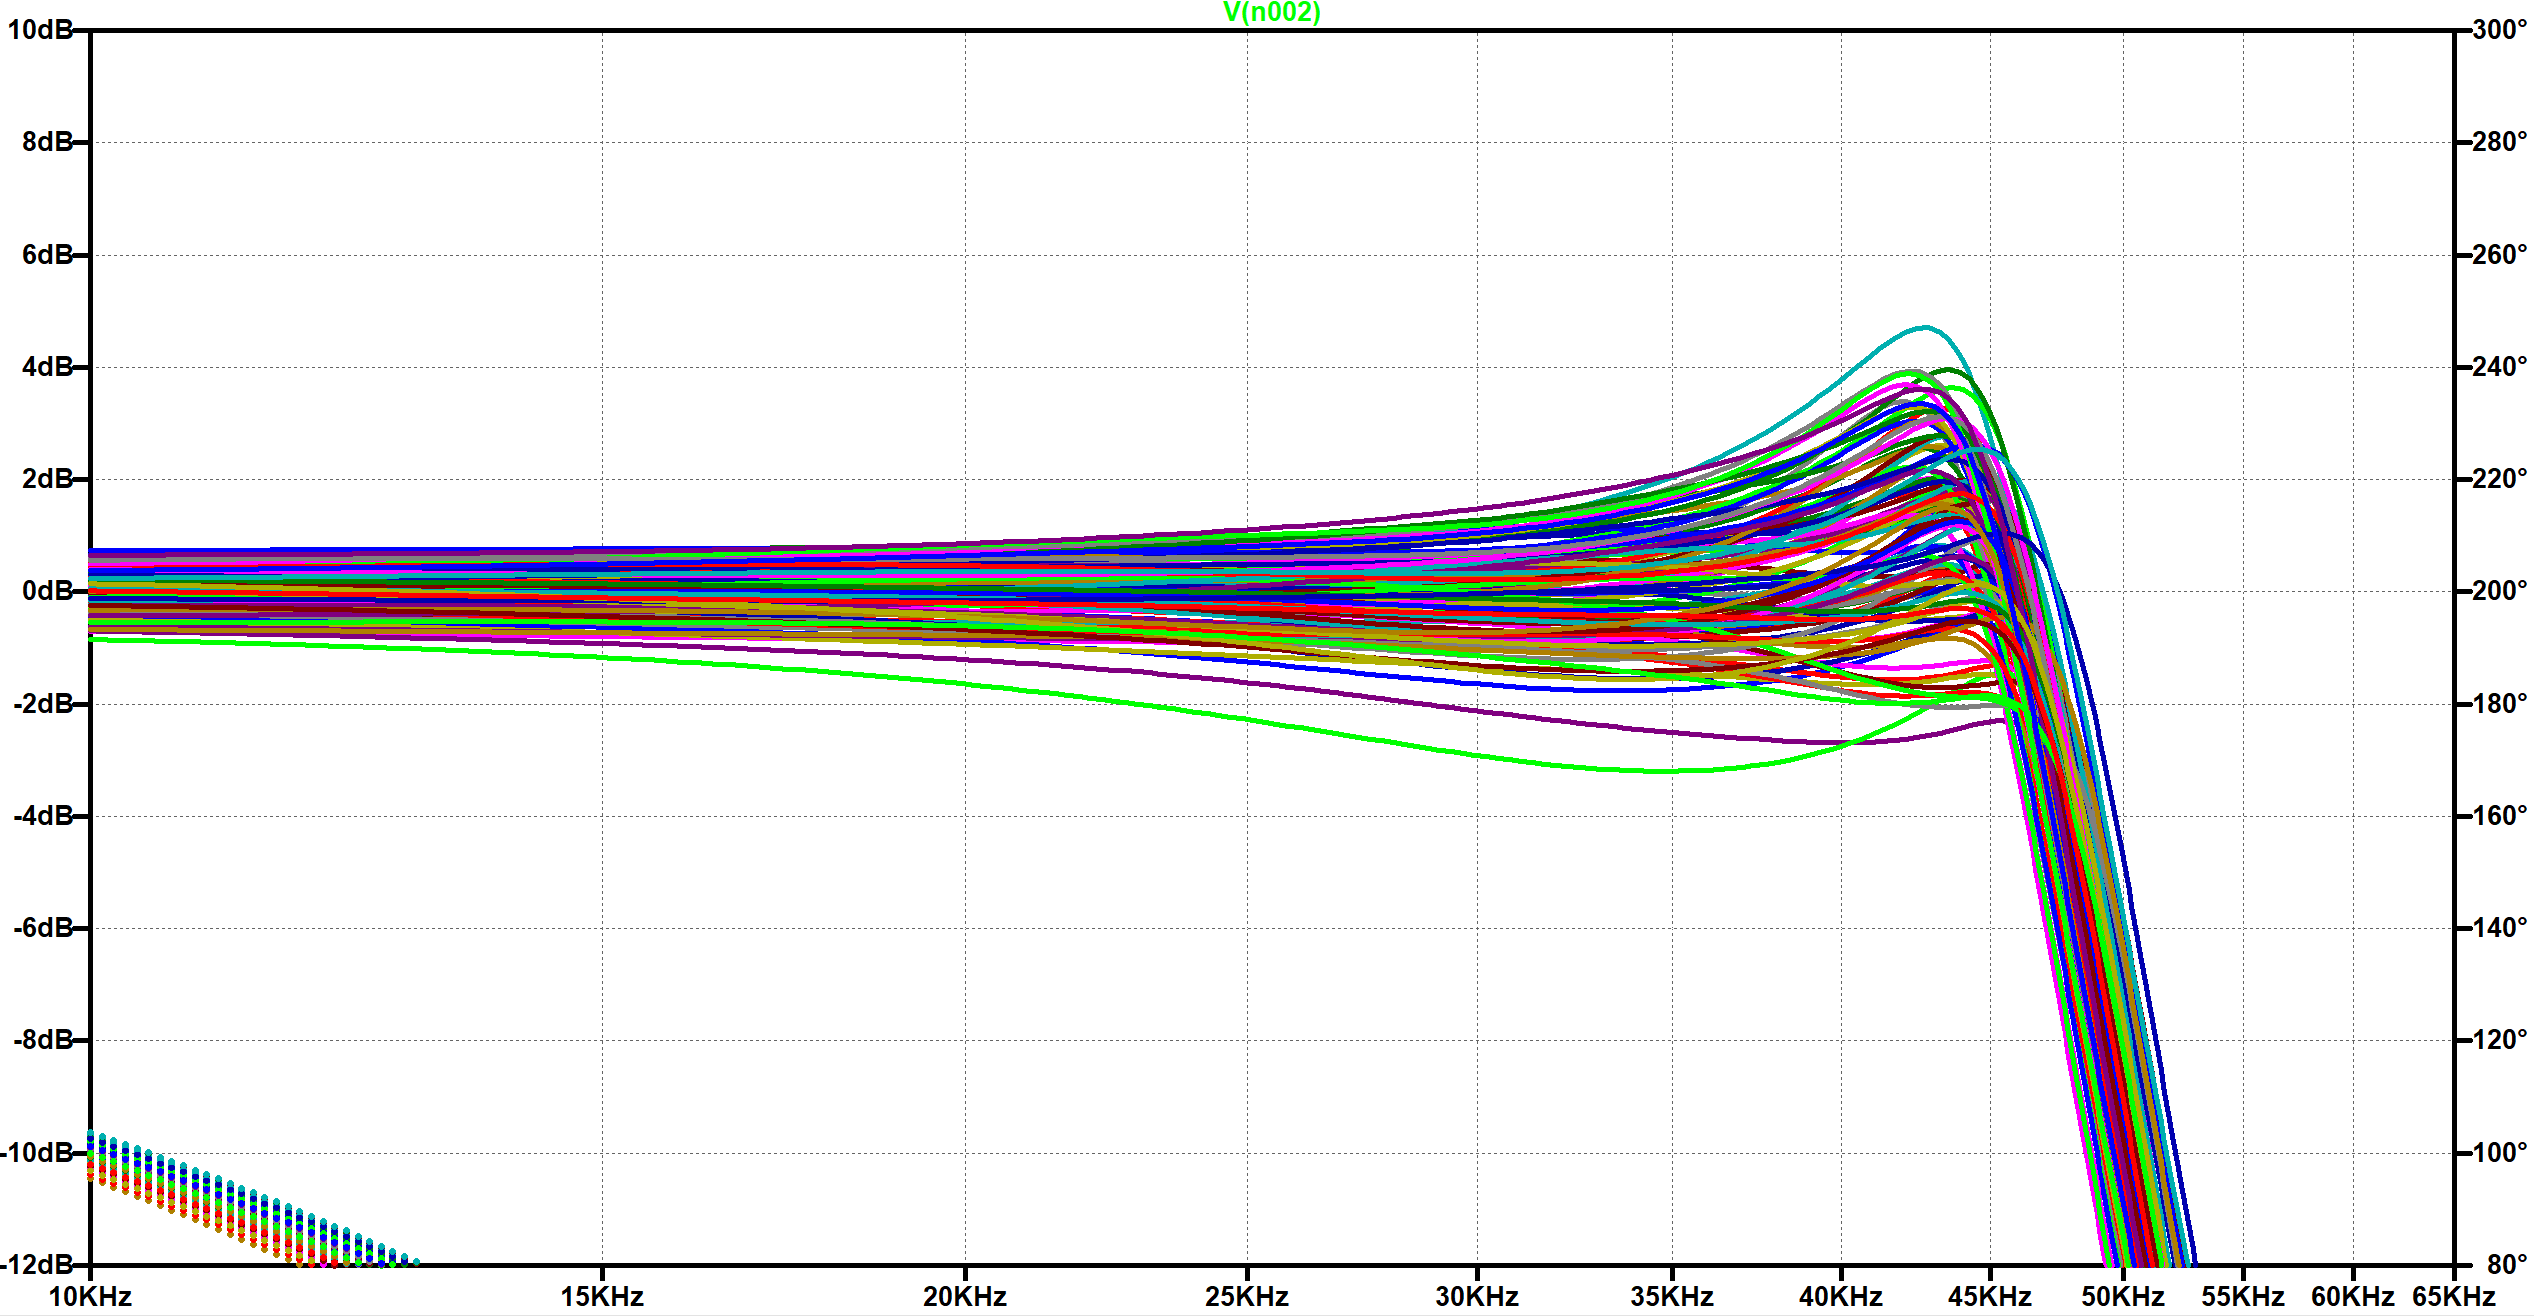
\includegraphics[scale=0.27]{Imagenes/CyR_al_5.PNG}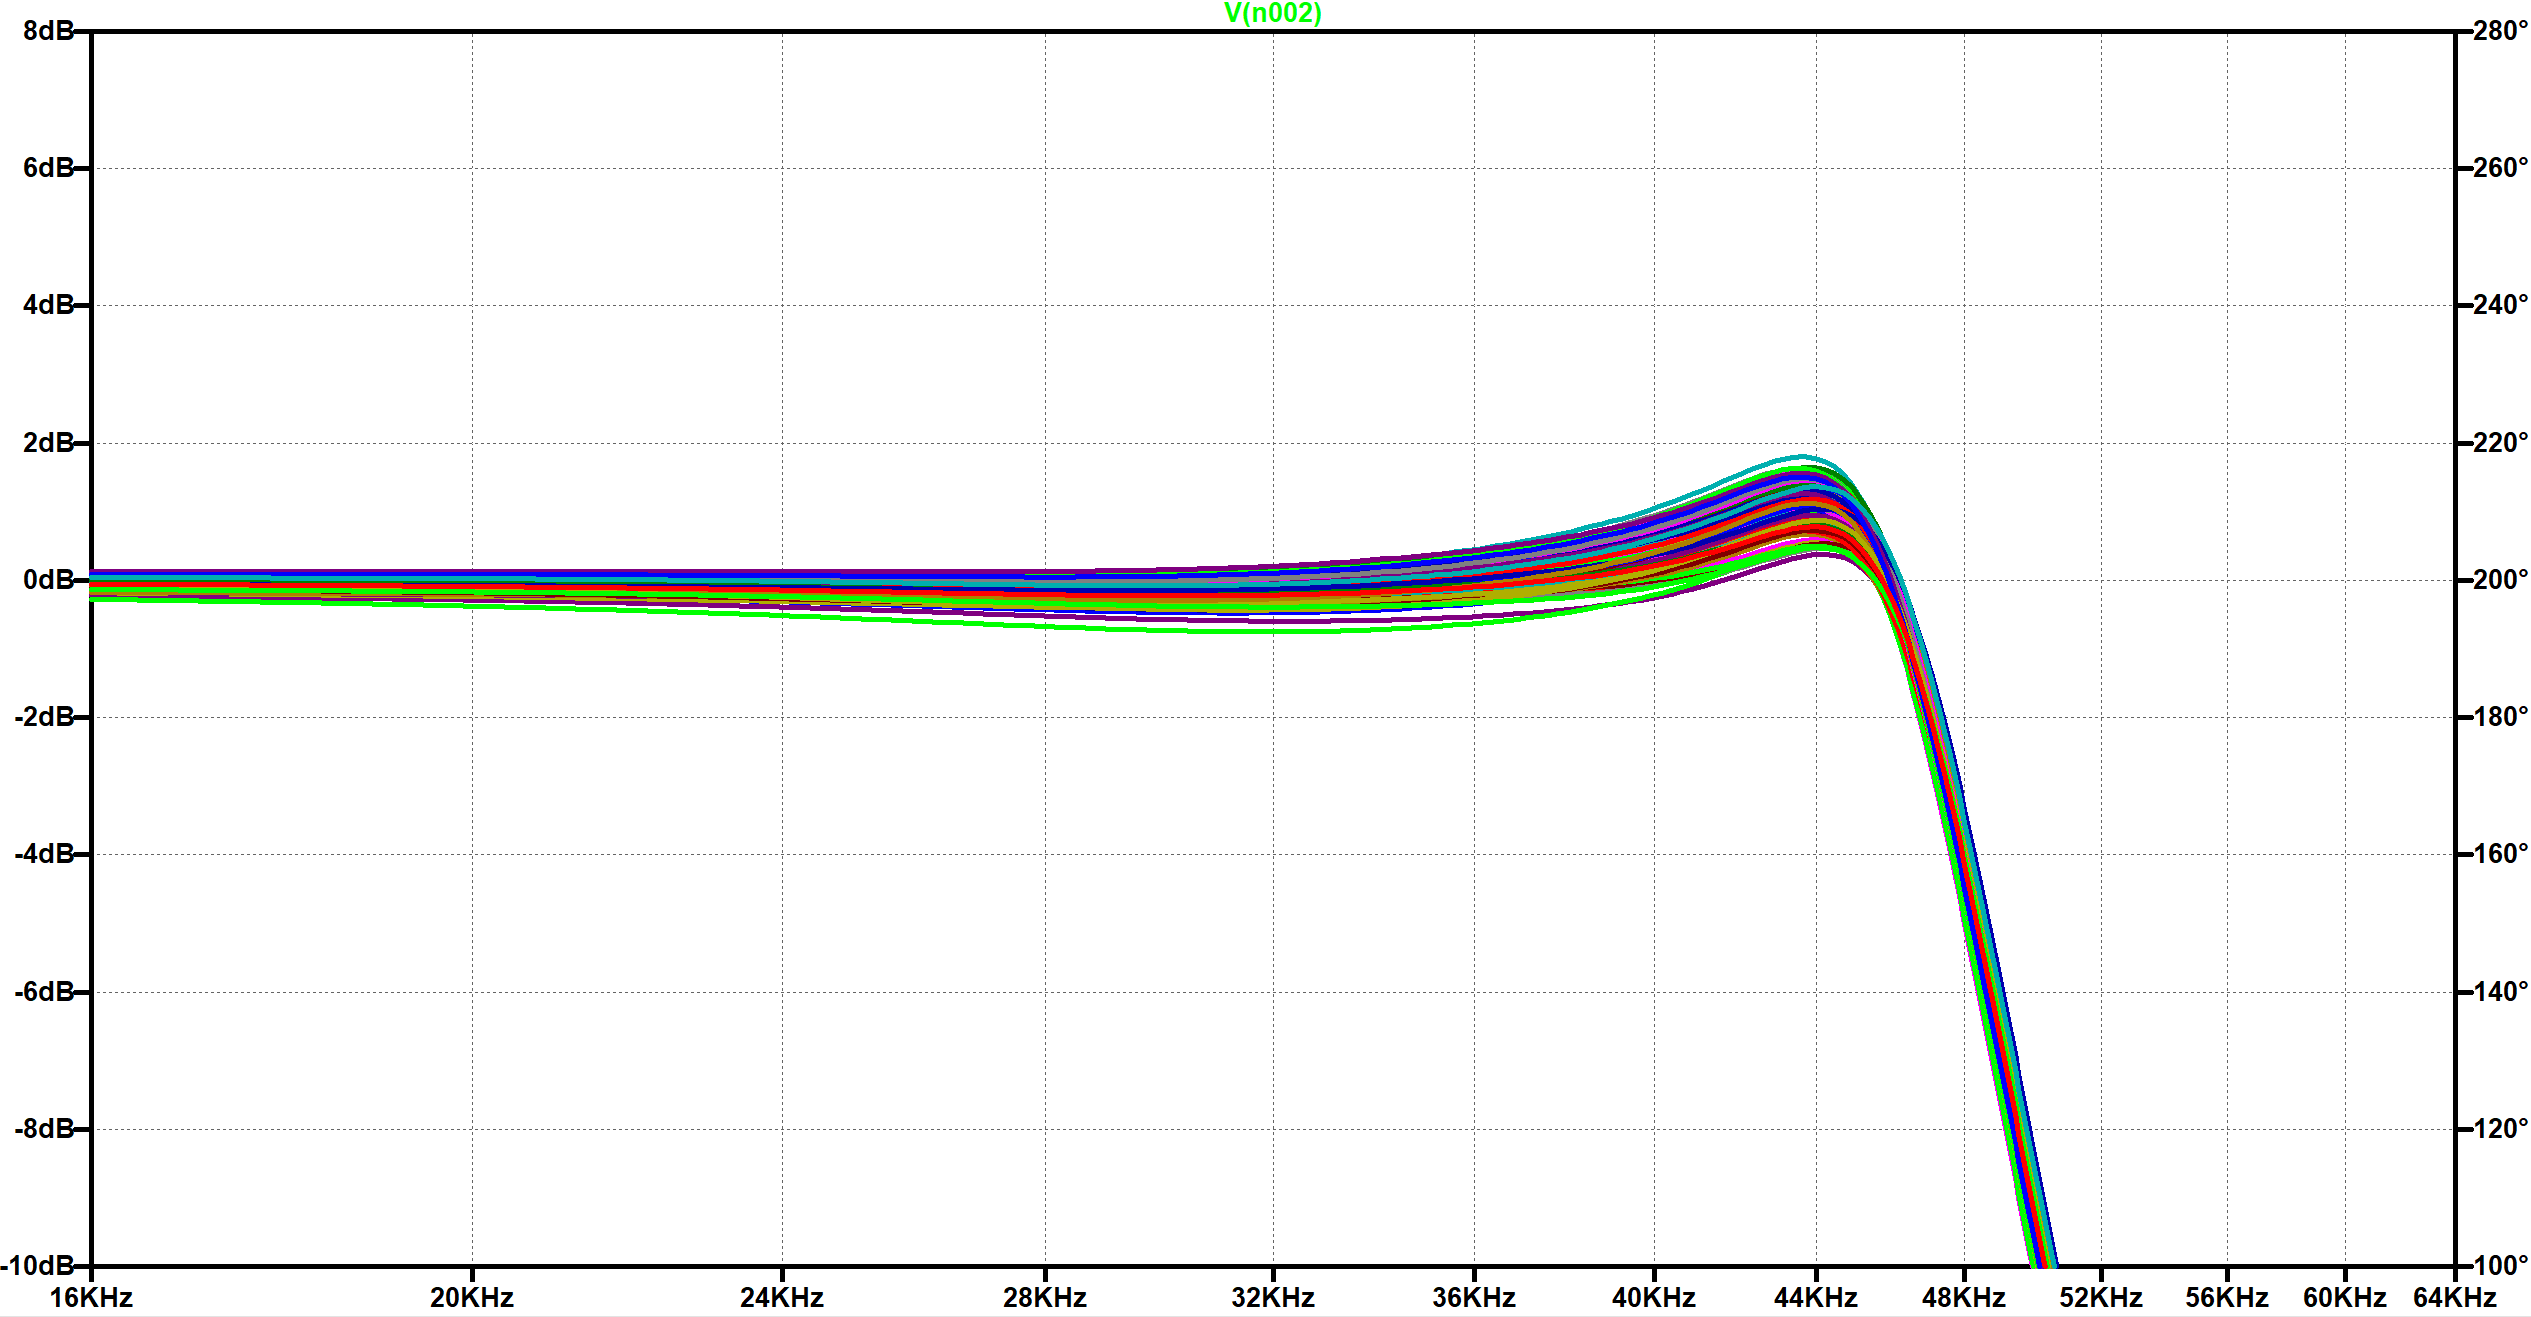
\includegraphics[scale=0.27]{Imagenes/CyR_al_1.PNG}


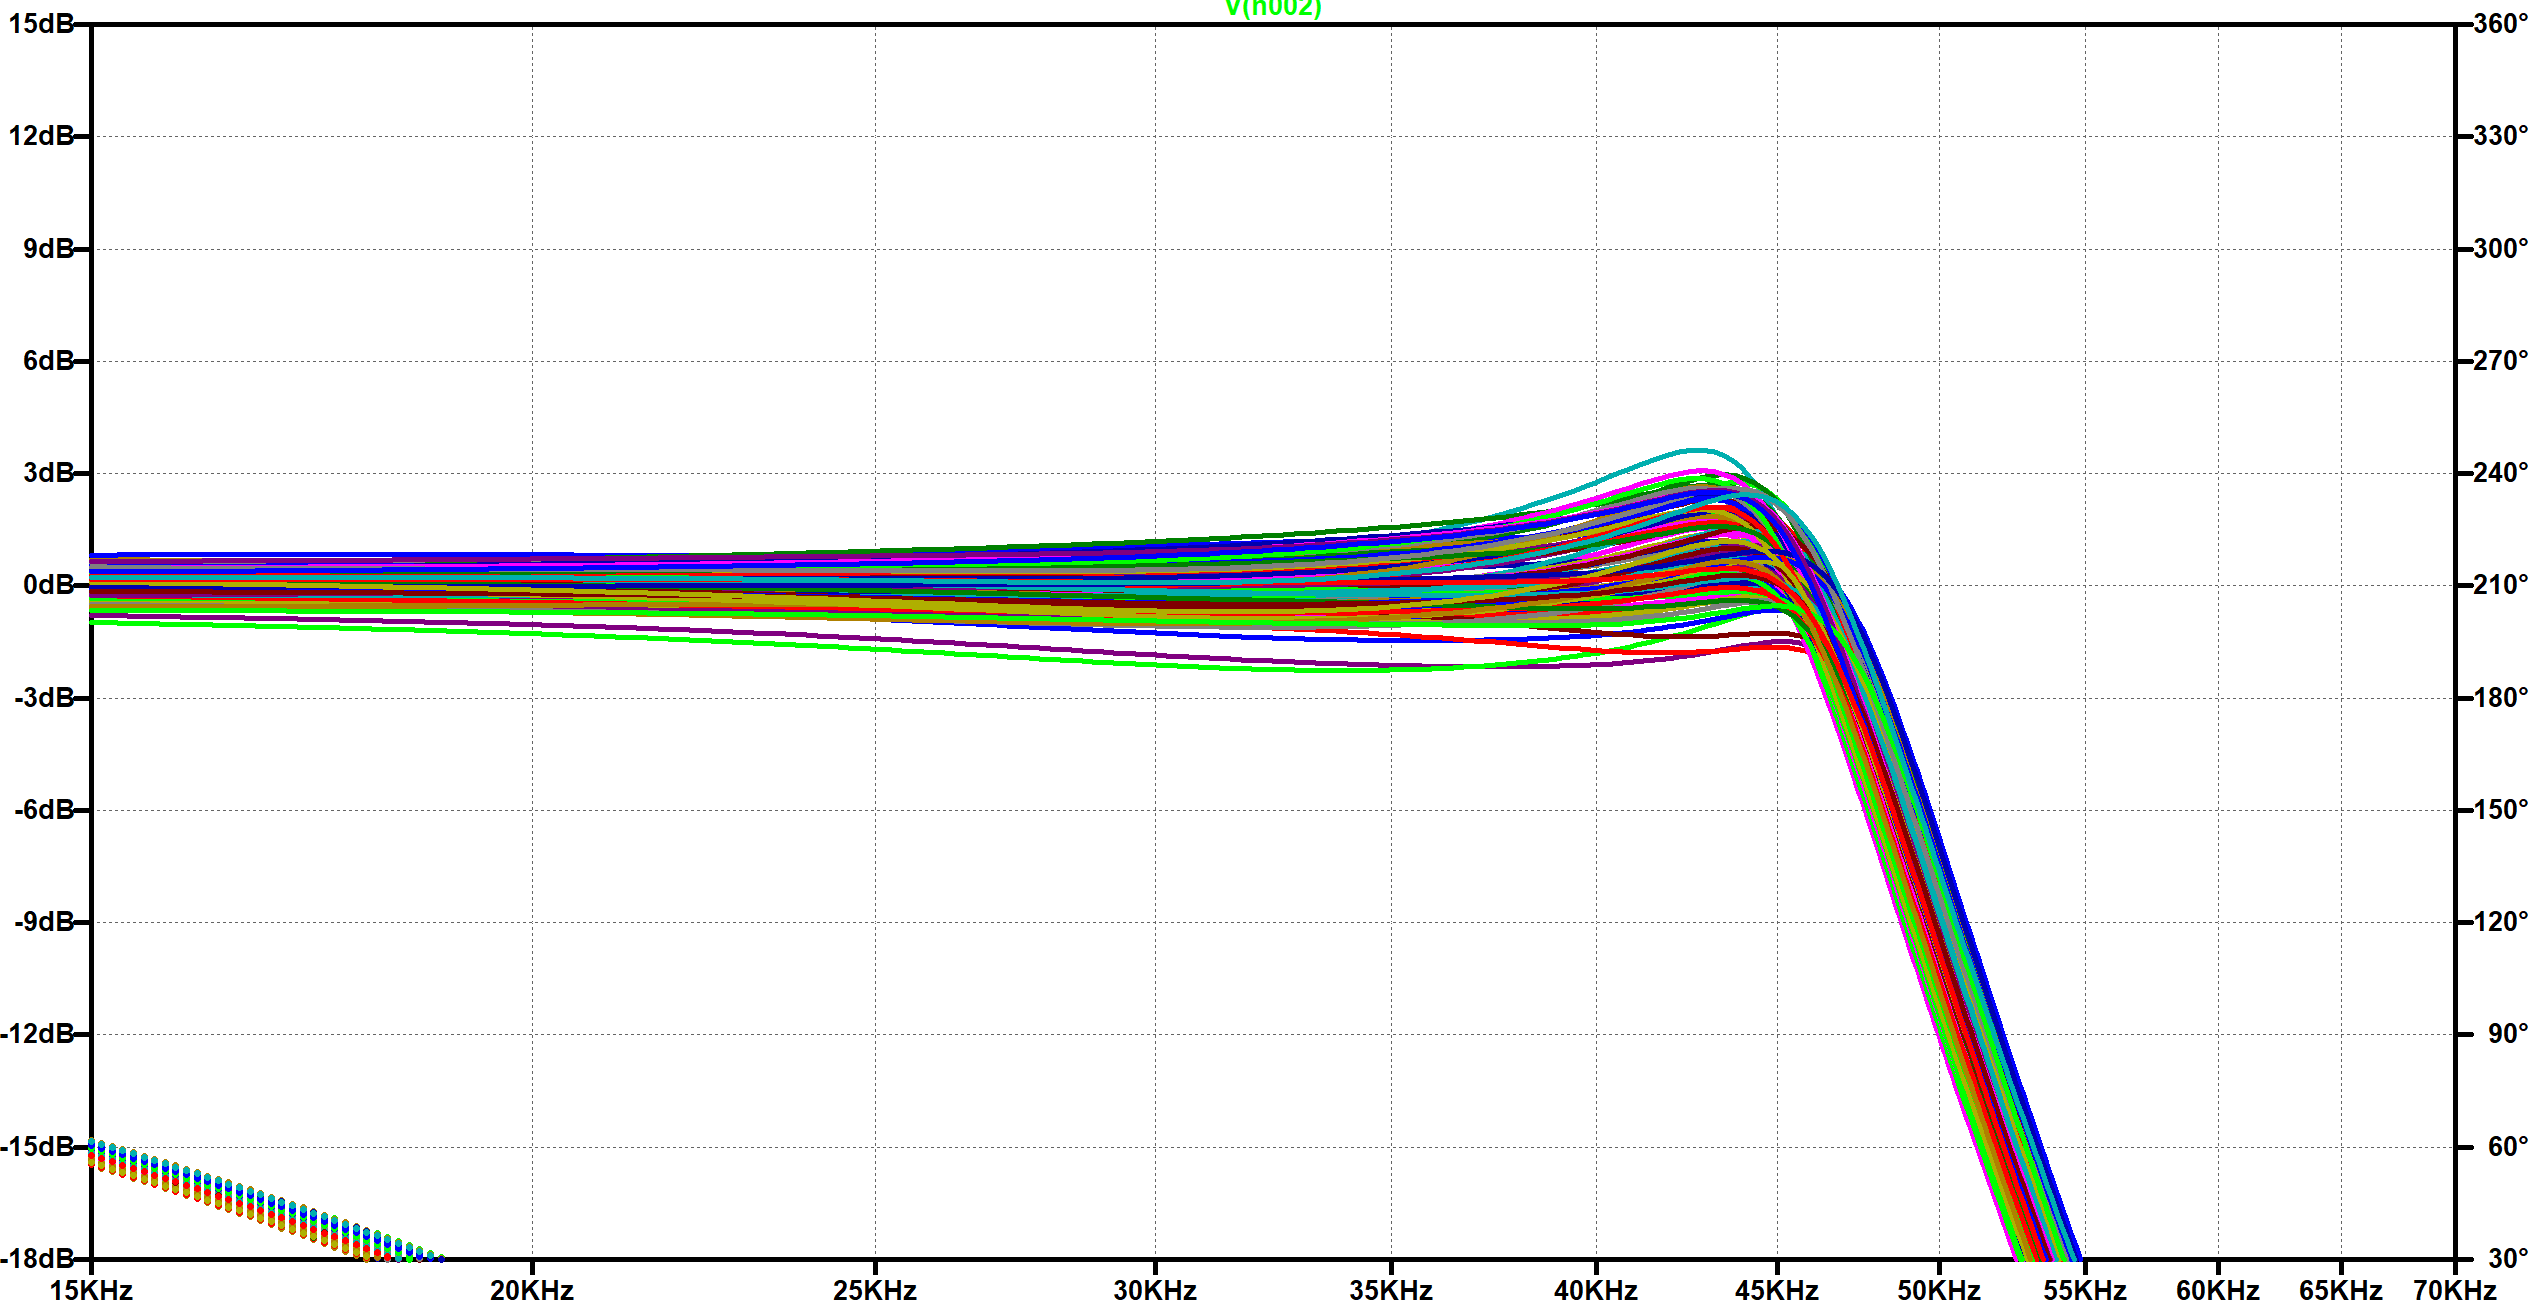
\includegraphics[scale=0.27]{Imagenes/C_al_1_yR_al_5.PNG}

\par\end{center}
\caption{De izq a der: C y R al 10\%, C y R al 1\%, C al 10\% y R al 1\%}
\label{fig:montecarlo}
\end{figure}



Gracias a este análisis, pudimos concluir que si bien los componentes
al 10\% nos arrojan una excesiva dispersión, los componentes que más
influyen en este aspecto son las resistencias, por lo que al utilizar
tecnología SMD con una tolerancia de 1\% nos aseguramos que el filtro
va a estar dentro de nuestra banda de tolerancia.

\subsection{Mediciones}
Una vez realizada la placa final, se procedió a realizar las mediciones pertinentes sobre el filtro en condiciones aisladas (es decir sin que otras etapas de la placa lo carguen). Se obtuvieron los siguientes resultados:

\begin{figure}[H]
\begin{center}
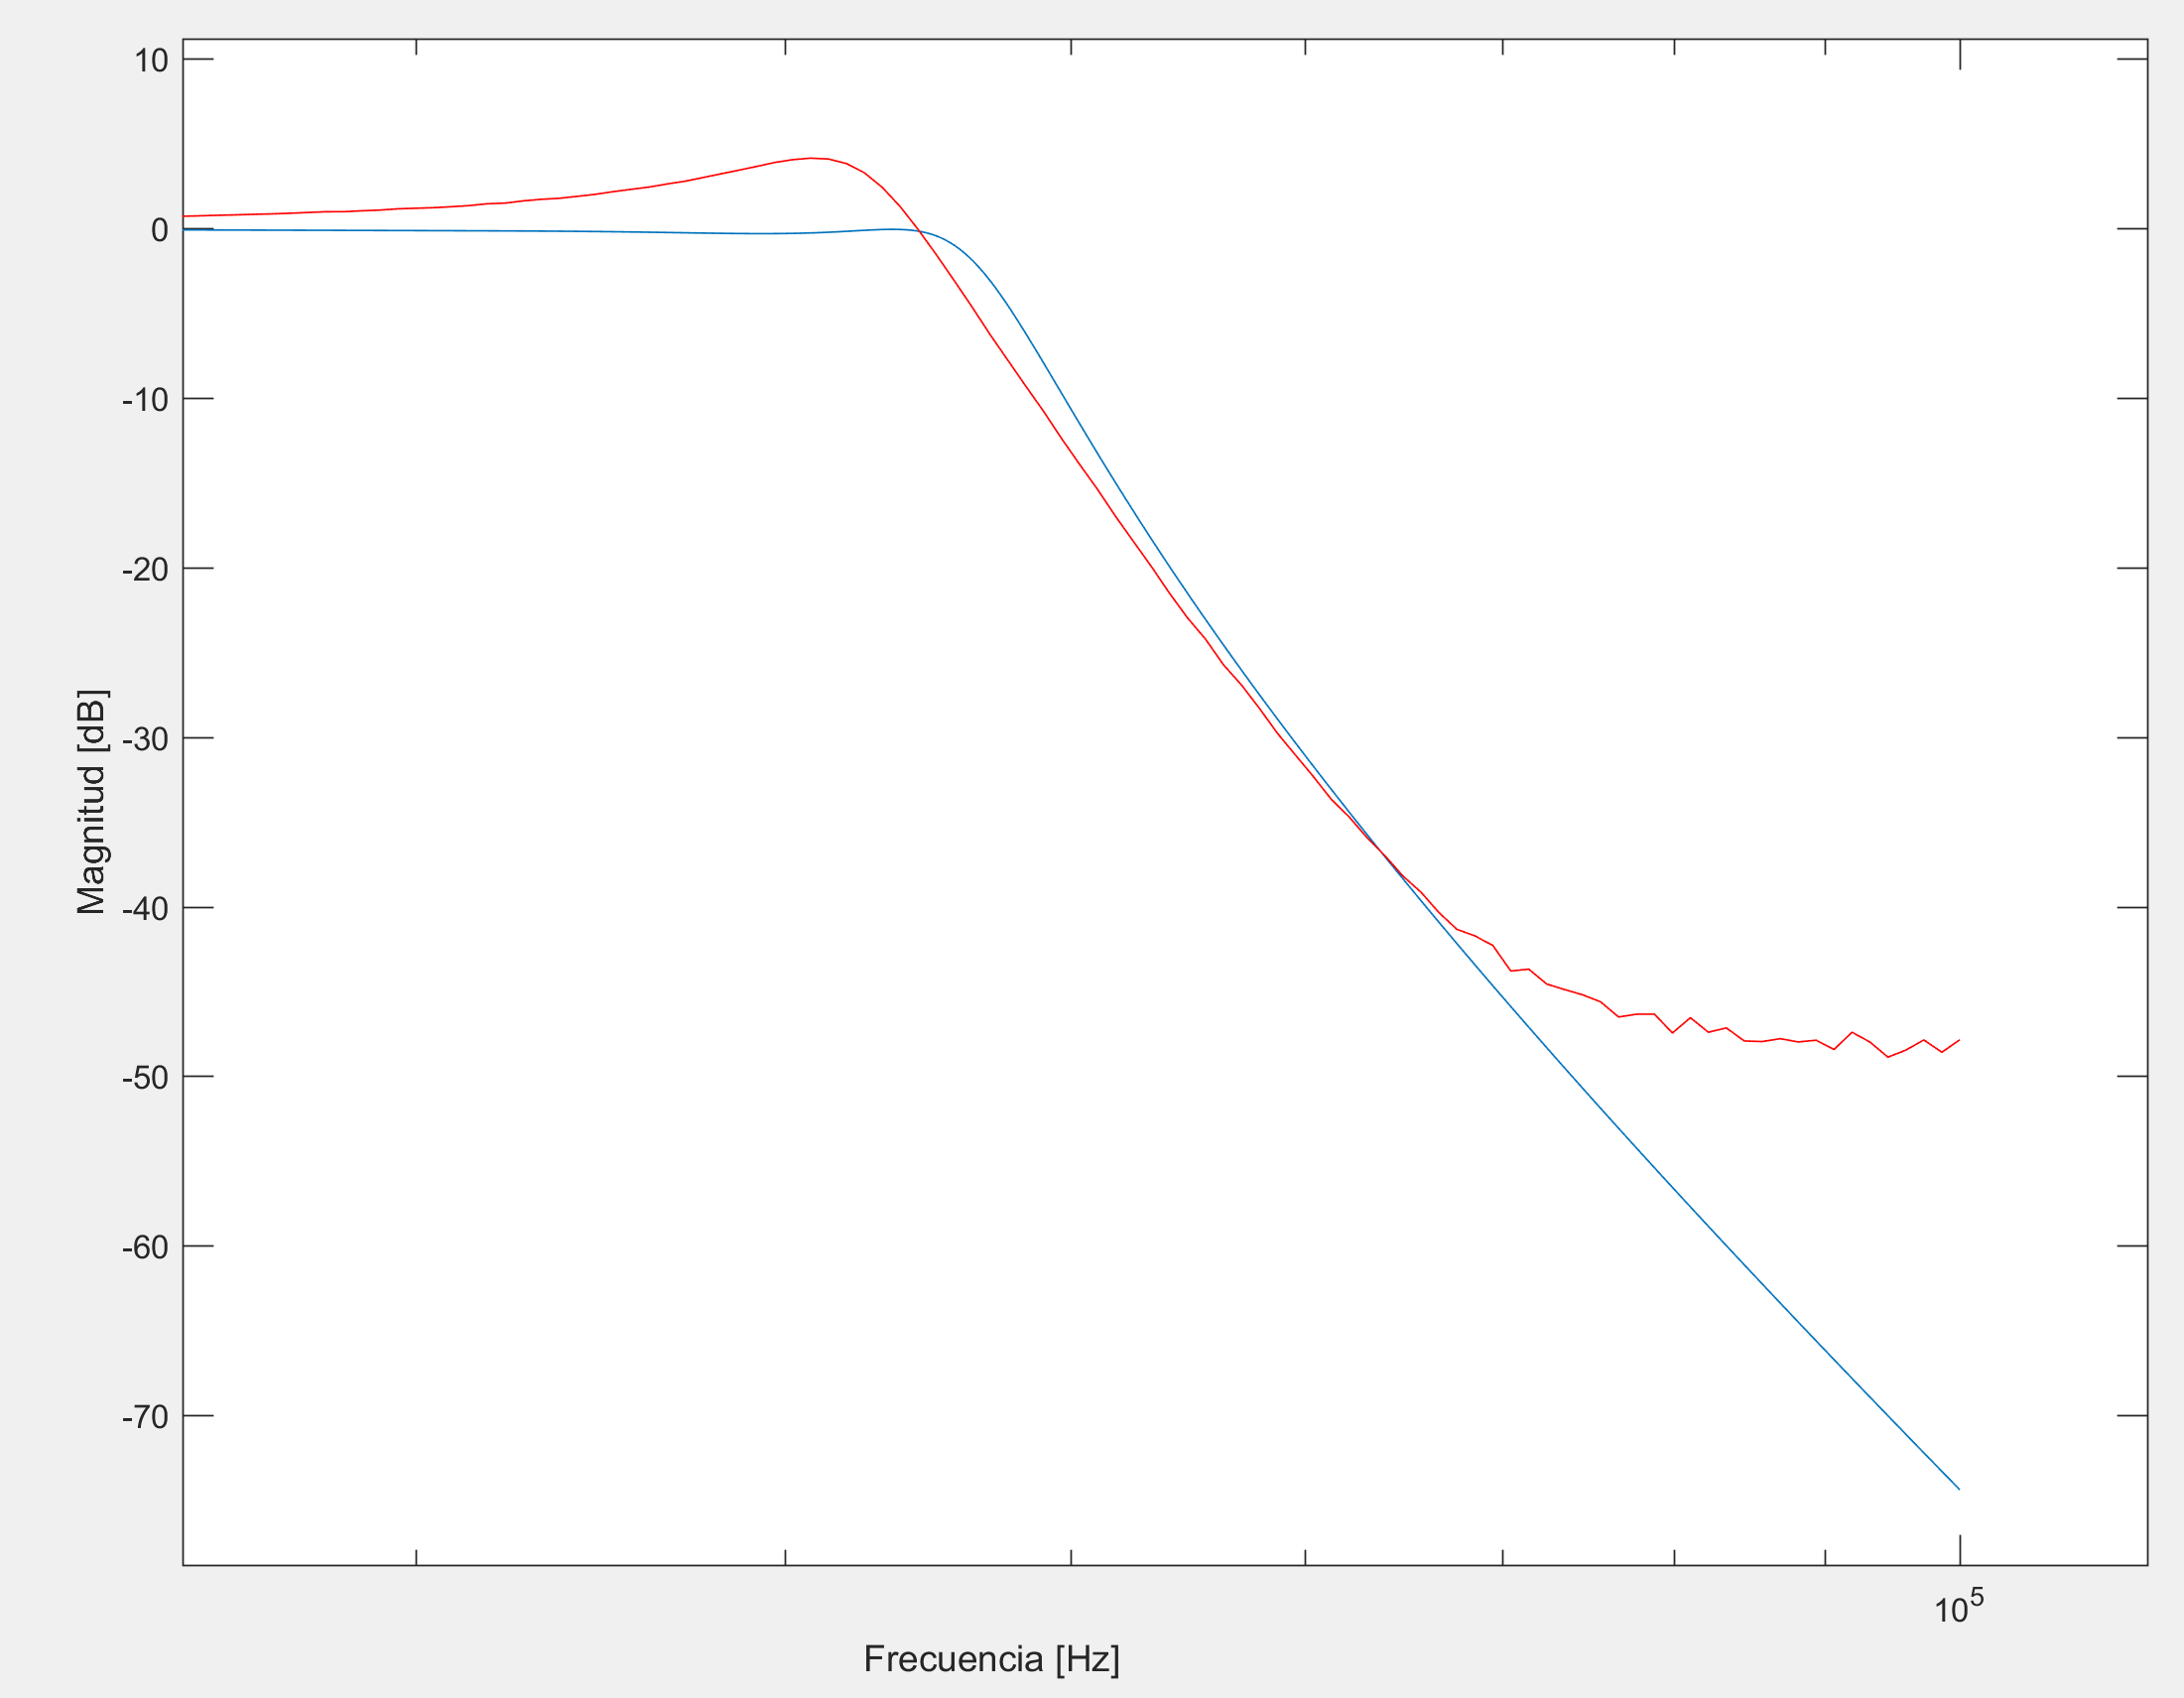
\includegraphics[scale=0.6]{Imagenes/bode.png}
\end{center}
\caption{En rojo, las mediciones obtenidas, en azul el filtro simulado.}
\end{figure}

Como podemos observar en la imagen, el filtro construido resultante no se comporta en absoluto a como el filtro ideal simulado, y si volvemos a mirar el análisis de montecarlo en la figura \ref{fig:montecarlo} vemos que tampoco entra en el rango predecido por dicho análisis. A pesar de tener presets para poder calibrar el filtro, no fue posible lograr una mejor medición que la que se muestra, por lo que vamos a proceder a enumerar las consecuencias de tener un filtro de dichas características:
\begin{itemize}
\item Las frecuencias que ingresen al filtro y que estén cercanas a la frecuencia de corte del mismo van a sufrir una amplificación haciendo que probablemente saturen en esa frecuencia.


\item Esa ganancia va a insertar una respuesta transitoria sobre mi señal de aproximadamente la frecuencia del filtro.

\item Los distintos armónicos que pasen por el filtro van a sufrir distintos desfasajes producto de la construcción de dicho filtro.
\end{itemize}


\end{document}
